\documentclass[../main.tex]{subfiles}

\newcommand{\cI}{\mathcal{I}}
\begin{document}

\section{OPEs from backreaction}\label{sec:br}

The correspondence between the theory on a stack of branes and the gravitational theory defined on the locus away from the brane is not an exact one, even at the twisted level: to obtain a match one must include effects from the backreaction.
Geometrically, the backreaction defines the sort of geometry which is dual to the theory on a large stack of branes.
This perspective persists for twisted holography.
Algebraically, and importantly for us, the backreaction has the effect of deforming the dual gravitational chiral algebra defined on the boundary of (twisted) $AdS$ space.

In this section, we proceed to compute planar corrections to the OPE which involve the backreaction. 
This will complete the determination of the planar limit of the holographically dual chiral algebra.

Since the integrals arising from diagrams this section are slightly more involved, we set up the following notations.
The holomorphic coordinate on $\C^3$ will be $Z = (z , w)$ where $w = (w^1,w^2)$ is a holomorphic coordinate on $\C^2$.
The defect will be located along $w = 0$.
In the formulas below, our convention is that $Z^0 = z$ and $Z^i = w^i$ for $i=1,2$.

Before getting into the main computation of the section, we turn our attention to a simpler example.

\subsection{Warmup: holomorphic Chern--Simons theory}

In this section, we warm up by computing the effect of backreaction on the open string sector only of a ``bulk'' theory. That is, we study how holomorphic Chern-Simons theory, which may be interpreted as the open string field theory for some space-filling branes in the bulk, deforms in the presence of a certain Kodaira-Spencer field (or Beltrami differential). 
More precisely, we consider holomorphic Chern--Simons in the presence of a Kodaira--Spencer field which is sourced by $N$ $D1$ branes wrapping $\C \subset \C^3$. 
The backreaction field is 
\[
\mu_{BR} = \frac{\eps_{ij} \wbar^i \d \wbar^j}{2 \pi \|w\|^4} \partial_z \in \PV^{1,1} (\C^3 \setminus \C) . 
\]
This field satisfies the equation
\beqn\label{eqn:csBR}
\dbar \mu_{BR} \wedge \Omega_{w_i=0} = N \delta_{w_i = 0} \del_z 
\eeqn
where $\delta_{w_i=0}$ is the $\delta$-function supported at $w_i=0$.
This couples to the holomorphic Chern--Simons field by 
\[
S_{BR} = \frac12 \int_{\C^3} \mu_{BR} \vee \op{tr}(A \del A) = \frac12 N \int_{\C^3} A^a \frac{\eps_{ij} \wbar^i \d \wbar^j}{2\pi \|w\|^4} \partial_z A^a .
\]
We will denote $\omega = \frac{\eps_{ij} \wbar^i \d \wbar^j}{2 \pi \|w\|^4}$ so that the coupling can be written $S_{BR} = \frac{N}{2}
\int_{\C^3} A \omega \del_z A.$

The backreaction coupling has a gauge anomaly even at tree-level.
Indeed, the tree-level gauge variation of $S_{BR}$ is
\[
\int_{\C^3} A^a (\dbar \mu_{BR}) \fc^a = \int_{\C_z} A_{\zbar}^a \partial_z \fc^a .
\]
In order to cancel this gauge anomaly one must introduce an $N$-dependent term in the OPE of the currents $J_a[k,l]$. 
In fact, at tree level only the OPE between currents with $k=l=0$ 
is affected by the tree-level backreaction.
In the presence of the backreaction the currents $J_a[0,0]$ form a Kac--Moody algebra of level $N$
\[
J_a[0,0] (0) J_b [0,0] (z) \simeq f_{ab}^c \frac1z J_c[0,0] + \delta_{ab} N \frac1{z^2} {\rm Id} .
\]
The second term in the OPE is present due the the existence of a tree-level anomaly which involves the back reaction.
The diagram which represents this anomaly is presented in figure \ref{fig:hcstreebr}.

\begin{figure}
	\begin{tikzpicture}	
			\node (A1) at (3,1) {};
			\node (A2) at (3,-1){};

		\node[circle,draw,fill=black]  (V1) at (1.5,0) {}; 
		\draw[decorate]  (V1) --  (A1);
		\draw[decorate] (V1) -- (A2);
		%\draw[decorate,decoration={snake}](0,-1) -- (V2);
		\draw[dashed] (0,0) -- (V1);

		\draw (0,2) -- (0,-2);	
		
	\end{tikzpicture}
	\label{fig:hcstreebr}
	\caption{Tree-level diagram involving the backreaction which contributes an anomaly.}  
\end{figure}

What about higher loop anomalies involving the backreaction?
For scaling dimension reasons, there are no further corrections to the $J[0,0]-J[0,0]$ OPE.
Let's consider the possibility of quantum corrections to the OPE between the fields $J_a[1,0]$ and $J_b[0,1]$. 
Before accounting for the back reaction, the tree and one-loop level OPE is 
\beqn\label{eqn:Jbr}
J_a[1,0](z) J_b[0,1] \simeq \frac{1}{z} f^c_{ab} J[1,1] + \hbar \frac1z K^{fe} f_{ae}^c f_{bf}^d J_c[0,0] J_d[0,0] ,
\eeqn
(see e.g. section 6 of \cite{CP}).
By conformal invariance, the possible $N$-dependent terms in the OPE $J_a[1,0] (0) J_b [0,1](z)$ must be of the form
\[
\alpha f^c_{ae} K^{be}  \left(\frac{1}{z^2} J_c[0,0] + \frac{1}{z} \del_z J_c[0,0] \right) + \beta K^{ab} \frac{1}{z^3} {\rm Id} 
\]
for some (possibly zero) constants $\alpha,\beta$ which depend on~$N$
(notice that the form of the central term in the last term is consistent with the fact that $J[1,0], J[0,1]$ are of spin $3/2$).
The diagrams which give rise to the anomalies necessitating these terms in the OPE are presented in figure \ref{fig:hcsloopbr}.
In these diagrams, the dotted lines represent coupling to the backreaction and the wiggle lines represent bulk propagators.
The straight lines label bulk field inputs, as before.

\begin{figure}
	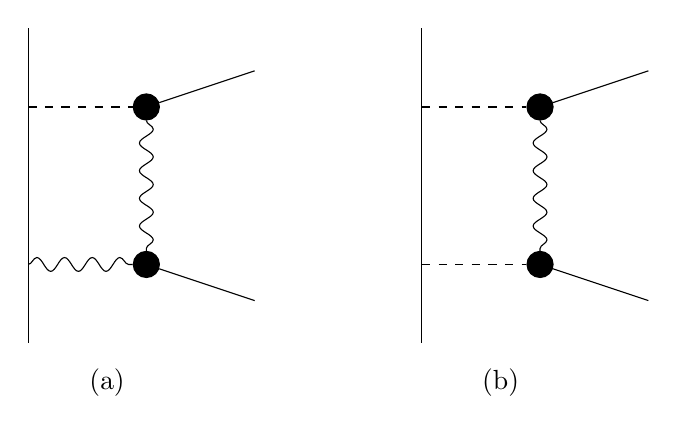
\begin{tikzpicture}
	\begin{scope}		
			\node (A1) at (3,1.5) {};
			\node (A2) at (3,-1.5){};

		\node[circle,draw,fill=black]  (V1) at (1.5,1) {}; 
		\node[circle,draw,fill=black]  (V2) at (1.5,-1) {};  
		\draw[decorate]  (V1) --  (A1);
		\draw[decorate, decoration={snake}] (V1) -- (V2);
		\draw[decorate] (V2) -- (A2);
		\draw[decorate,decoration={snake}](0,-1) -- (V2);
		\draw[dashed] (0,1) -- (V1);

		\draw (0,2) -- (0,-2);	
		
		\node[] at (1,-2.5) {(a)};
		
	\end{scope}

		\begin{scope}[shift={(5,0)}]		
			\node (A1) at (3,1.5) {};
			\node (A2) at (3,-1.5){};

		\node[circle,draw,fill=black]  (V1) at (1.5,1) {}; 
		\node[circle,draw,fill=black]  (V2) at (1.5,-1) {};  
		\draw[decorate]  (V1) --  (A1);
		\draw[decorate, decoration={snake}] (V1) -- (V2);
		\draw[decorate] (V2) -- (A2);
		\draw[dashed](0,-1) -- (V2);
		\draw[dashed] (0,1) -- (V1);

		\draw (0,2) -- (0,-2);	
		
		\node[] at (1,-2.5) {(b)};
	\end{scope}
	\end{tikzpicture}
	\label{fig:hcsloopbr}
	\caption{One-loop diagrams involving the backreaction which contribute an anomaly.}  
\end{figure}

To evaluate the integrals associated to these diagrams we use point splitting on the defect so that operators are placed at $z_1$,$z_2 \in \C$ with $|z_1-z_2| \geq \epsilon$.
The edges of the diagram correspond to the propagator for the free part of holomorphic Chern--Simons theory, which is determined by the parametrix for the $\dbar$-operator on $\C^3$:
\beqn
(\dbar P) \wedge \d^3 Z = \delta_{Z=0} .
\eeqn
Explicitly, this is the $(0,2)$-form
\beqn\label{eqn:propagatorCS}
P(Z) = \frac{1}{4 \pi^2 r^6} \ep_{ijk} \br Z^{i} \d \br Z^j \d \br Z^k .
\eeqn

We first focus on diagram \ref{fig:hcsloopbr} (b).
The weight is represented by the integral
\beqn
\int_{(X,Y)} A_1(X) \, \omega (x) \,  \del_z \del_w P(X,Y) \, \omega(y) \, A_2(Y) ,
\eeqn
where we use coordinates $X = (x_1,x_2,z), Y = (y_1,y_2,w)$ and impose a cutoff $|z-w| \geq \epsilon$.
In appendix \ref{appx:hcsbr} we evaluate this integral to obtain
\beqn
\frac{N^2}{2} K_{ab} \ep_{ij} \int_{|z-w| \geq \epsilon} \frac{1}{(z - w)^3} \del_{w_i} A^a_1 \del_{w_j} A^b_2 |_{w_i=0},
\eeqn
where $A_1,A_2$ are the input gauge fields.
The linear BRST variation $A \mapsto A + \dbar c$ of this diagram thus gives rise to the anomaly
\beqn
\frac{N^2}{2} K_{ab} \ep_{ij} \int_{|z-w| \geq \epsilon} \frac{1}{(z-w)^3} \del_{w_i} A^a \del_{w_j} \dbar c^b |_{w_i=0}
\eeqn
Integrating by parts and taking $\epsilon \to 0$ this becomes
\beqn
\frac{N^2}{2} K_{ab} \ep_{ij} \del^3 \delta_{z_1=z_2} \del_{w_i} A^a \del_{w_j} \dbar c^b |_{w_i=0} .
\eeqn
In this form it is clear that this anomaly is canceled by introducing the term in the OPE in \eqref{eqn:Jbr} with
\beqn
\beta = \frac{N^2}{2} .
\eeqn




\subsection{Tree-level backreaction in Kodaira--Spencer theory}\label{sec:treebr}

We now turn to the effects of backreaction in our version of Kodaira--Spencer theory obtained by compactifying the twist of type IIB supergravity on a $K3$ surface.

The first nontrivial contribution from the backreaction actually occurs at tree-level, and is represented by Diagram b) in Figure \ref{fig:alldiagramsplanar}. We will determine this diagram first. 
Part of this contribution was computed in \cite{CP}.
The backreaction field $\mu_{BR} = \mu_{BR}(\bfeta)$ takes a similar form as in the previous section.
It is a distributional section
\beqn
\mu_{BR} \in \PV^{1,1}(\C^3) \otimes R
\eeqn
which satisfies the defining distributional equation
\beqn
\dbar \mu_{BR} = \delta_{w_i=0} F \del_z ,
\eeqn
where $F \in H^2(K3) \subset A$ is the flux labeling the brane configuration.

The field $\mu_{BR}$ couples to the fields $\mu_i$ via
\beqn\label{eqn:brmu1mu2}
\int_{Z,\bfeta} \mu_{BR} \mu_1  \mu_2
\eeqn
It couples to the fields $\alpha ,\gamma$ through
\beqn\label{eqn:brag}
\int_{Z,\bfeta} \mu_{BR} \alpha \del_z \gamma .
\eeqn
Notice that by type reasons the backreaction field does not couple to the Beltrami field~$\mu_z$ in the direction parallel to the brane.

We first consider the gauge anomaly involving the coupling \eqref{eqn:brmu1mu2}. 
The tree-level gauge variation of the backreaction coupling \eqref{eqn:brmu1mu2} is
\beqn\label{eqn:brtreeanomaly1}
\int_{Z,\bfeta} \mu_{BR} \dbar \lie{c}_1  \mu_2 +  \int_{Z,\bfeta} \mu_{BR}  \mu_1  \dbar \lie{c}_2 = \int_{z,\bfeta} \left(\lie{c}_1 \mu_2 + \mu_1 \lie{c}_2\right)|_{w = 0} .
\eeqn
Similarly, the tree-level gauge variation of the coupling \eqref{eqn:brag} is 
\beqn\label{eqn:brtreeanomaly2}
\int_{Z,\bfeta} \mu_{BR} \dbar \lie{c}_\alpha  \del_z\gamma  +  \int_{Z,\bfeta} \mu_{BR}  \alpha  \dbar \del_z\lie{c}_\gamma = \int_{z,\bfeta} \left(\lie{c}_\alpha \del_z \gamma + \alpha \del_z\lie{c}_\gamma\right)|_{w = 0} .
\eeqn

Notice that neither of these expression involve $w_i$-derivatives. 
Since $\til{J}^i[0,0]$ couples to $\mu_i$, the anomaly in \eqref{eqn:brtreeanomaly1} can be cancelled by the gauge variation of 
\beqn
\int_{z,\bfeta,z',\bfeta'} \til{J}^1[0,0](z) \mu_1(z) \til{J}^2[0,0] (z') \mu_2(z')
\eeqn
provided that the $\til{J}^i[0,0]$ operators satisfy an appropriate OPE. 
Similarly, the anomaly in \eqref{eqn:brtreeanomaly2} can be cancelled by the gauge variation of a coupling of the form
\beqn
\int_{z,\bfeta,z',\bfeta'} G_\alpha[0,0](z) \alpha(z) G_\gamma[0,0] (z') \gamma (z') .
\eeqn

Proceeding as above by working in the Fourier dual odd coordinates and then transforming to the basis of on-shell fields, we see that to cancel the first of these anomalies there must be a term in the off-shell $\til J \til J$ OPE of the form
\beqn
\til{J}^i[0,0](0,\what\bfeta) \til{J}^j [0,0] (z,\what\bfeta') \simeq \ep^{ij} \frac1z \what F (\what\bfeta + \what\bfeta') .
\eeqn
Using the constraints \eqref{eqn:onshell} we can write this OPE in terms of on-shell fields as
\beqn
J[1,0](0,\what \bfeta) J[0,1] (z,\what \bfeta') \simeq \frac{1}{z} \what F(\what \bfeta + \what \bfeta') .
\eeqn
To cancel the second anomaly \eqref{eqn:brtreeanomaly2} there must be a term in the $GG$ OPE of the form
\beqn
G_\alpha[0,0](0,\what \bfeta) G_\gamma[0,0](z,\what \bfeta'\\) \simeq \frac1{z^2} \what F (\what \bfeta + \what \bfeta') .
\eeqn

Recall that in section \ref{s:sugraelliptic} we pointed out a discrepancy in our supergravity elliptic genus and the one computed in \cite{deBoerEG}, which in the notation of that section arose from the two representations $(\frac{\bf 1}{\bf 2})_S \otimes H^{2,0}(K3)$ and $(\frac{\bf 1}{\bf 2})_S \otimes H^{2,2}(K3)$.
We observe that these representations form a sub-chiral algebra. 
%\natalie{Check the following... does this account precisely for all these chiral algebra generators/OPEs?} In particular, it recovers the twist of the fields in the $U(1)$ supermultiplet that corresponds to the collective motion of the $D1-D5$ system in the transverse directions $\C^2$.
Indeed, if we expand $J[1,0]$ in the Fourier dual coefficients as
\beqn
J[1,0](\what \bfeta) = J_0[1,0] + \what \eta J_{\what \eta} [1,0] + \cdots ,
\eeqn
and similarly for $J[0,1]$, then these representations correspond to the fields 
\beqn
J_0 [1,0],J_{\what \eta}[1,0],J_0 [0,1],J_{\what \eta}[0,1] .
\eeqn
The only OPEs between these fields involves the flux $F$.
They are given by
\begin{align*}
J_0 [1,0](0) J_{\what \eta} [0,1] (z) \simeq \frac{\br f}{z}  \\ 
J_0[0,1] (0) J_{\what \eta} [1,0] (z) \simeq - \frac{\br f}{z} 
\end{align*}
where $\br f$ is the component of $\br \bfeta$ in the original flux $F \in H^2(K3)$.

Consider next the operators 
\[
J[1,0](\what \bfeta), J[0,1](\what \bfeta),G_\alpha[0,0](\what \bfeta), G_\gamma[0,0](\what \bfeta) .
\]
These operators form a subalgebra of the full gravitational chiral algebra, even after taking into account the effect of the backreaction.
%Indeed, the $JG$ OPE's for this class of operators vanish.
We can relate this to a familiar system of free fields by a simple modification.
Recall that the spin of the operator $G_\alpha[0,0]$ is one.
If we choose a spin zero operator $\til G_{\alpha}[0,0]$ such that $\del \til G_\alpha [0,0]$ then we can obtain the same OPE as above if we declare that 
\beqn
\til G_\alpha[0,0](0,\what \bfeta) G_\gamma[0,0](z,\what \bfeta') \simeq \frac1{z} \what F (\what \bfeta^a + \what \bfeta'^a) .
\eeqn
The operators $J[1,0](\what \bfeta), J[0,1](\what \bfeta),\til G_\alpha[0,0](\what \bfeta), G_\gamma[0,0](\what \bfeta)$ form a familiar chiral algebra of free fields. 
The zero mode of $\til G$ is topological and can be ignored; the fact that we take the derivative arises in Kodaira-Spencer theory from the fact that we chose a potential for the corresponding polyvector field in \S \ref{sec:sugra}).

Explicitly, this is the $\beta \gamma bc$ system defined over the ring $R$. 
This is the chiral algebra whose fields (of spins 0,1,1/2,1/2 respectively)
\beqn
c = \til G_\alpha[0,0], b = G_\gamma [0,0], \beta = J[1,0] , \gamma = J[0,1]
\eeqn
are each valued in $R$.

From the point of view of the UV gauge theory, this comes from the twist of the fields in the $U(1)$ supermultiplet that corresponds to the collective motion of the $D1-D5$ system in the transverse directions. We emphasize that while these center of mass operators do have nontrivial OPEs with the remaining part of the chiral algebra, the operators which do not include the center of mass operators form a subalgebra of our holographically dual chiral algebra; recall that the contribution of these center of mass operators was subtracted by hand in \S \ref{sec:enumerate} to match the elliptic genus of \S \ref{sec:CFT}.
%The twist is $R$-valued because the target space directions corresponding to the center of mass degrees of freedom include an additional factor of $X =K3, T^4$ from the D5-brane worldvolume gauge theory (in the $T^4$ case, these degrees of freedom can be understood simply as Wilson lines on the homology cycles \cite{Davidetal}).


\subsection{The propagator for Kodaira--Spencer theory}

In a moment we will proceed with the characterization of how higher loop effects involving the backreaction in the $K3$ version of Kodaira--Spencer theory deforms the boundary chiral algebra.
To set up the computations we recall the form of the propagator in Kodaira--Spencer theory.
In this section we follow \cite{CLbcov1}.

The propagator for Kodaira--Spencer theory on $\C^3$ is the kernel for the operator $\del \dbar^* \tr^{-1}$. 
We obtain this by applying the divergence operator to the kernel for the operator $\dbar^* \tr^{-1}$ (the analytic part of this kernel is the same as the analytic part of the propagator used in holomorphic Chern--Simons theory). 
%Let us first recall the construction of the kernel for $\dbar^* \tr^{-1}$.

As usual, we use $Z = (Z_1 = w_1, Z_2=w_2,Z_3=z)$ for the holomorphic coordinate on $\C^3$.
Using the Calabi--Yau form one can express the integral kernel for the operator $\dbar^* \tr^{-1}$ in terms of the distributional Kodaira--Spencer field
\beqn
P(Z) = \frac{1}{4 \pi^2 r^6} \ep_{ijk} \br Z^{i} \d \br Z^j \d \br Z^k \del^3,
\eeqn
where $\del^3 = \del_{Z_1} \del_{Z_2} \del_{Z_3}$.
%This is a smooth section of $\PV^{3,2}(\C^3)$ away from $0 \in \C^3$.
The kernel is obtained by pulling back this section along the difference map 
\[
\C^3 \times \C^3 \to \C^3,\quad (Z,Z') \mapsto Z - Z' .
\]
We denote the pulled back section by
\[
P(Z,Z') \in \br{\PV}^{3,2}(\C^3 \times \C^3) . 
\]
Here $\br{\PV}^{3,2}$ stands for distributional Dolbeault valued polyvector fields of type $(3,2)$.
Notice that this section is smooth away from the diagonal in $\C^3 \times \C^3$. 

We are interested in the Kodaira--Spencer propagator which we will denote by $\bf P$; this is the kernel of the operator $\del \dbar^* \triangle^{-1}$. 
To obtain this, we first apply the divergence operator to $P$ 
\[
\bP = \del P \in \br\PV^{2,2}(\C^3) .
\]
Explicitly this is
\beqn
\bP (Z) = \frac{3}{4 \pi^2 r^8} \ep_{ijk} \ep_{lmn} \br Z^{i} \br Z^l \d \br Z^j \d \br Z^k \del_{Z_m} \del_{Z_n} .
\eeqn
We can expand this in terms of the coordinates $Z = (z,w_1,w_2)$ where $z$ is the holomorphic coordinate along the defect.
Then, 
\begin{align*}
P(z,w_i) = & \pm \frac{\d \wbar_1 \d \wbar_2}{r^8} \left(\zbar^2 \partial_{w_1} \partial_{w_2} - \zbar \br w_1 \partial_z \partial_{w_2} + \zbar \br w_2 \partial_z \partial_{w_1} \right) \\ 
& \pm \frac{\d \wbar_2 \d \zbar}{r^8} \left(\zbar \wbar_1 \partial_{w_1} \partial_{w_2} - \wbar_1^2 \partial_z \partial_{w_2} + \wbar_1 \wbar_2 \partial_z \partial_{w_1}\right) \\
& \pm \frac{\d \zbar \d \wbar_1}{r^8} \left(\zbar \wbar_2 \partial_{w_1} \partial_{w_2} - \wbar_1 \wbar_2 \partial_z \partial_{w_2} + \wbar_2^2 \partial_z \partial_{w_1} \right) .
\end{align*}

Pulling back along the difference map we obtain the Kodaira--Spencer theory propagator
\[
\bP (Z,Z') \in \br\PV^{2,2}(\C^3 \times \C^3) .
\]
This distribution is the integral kernel for the operator $\partial \dbar^* \tr^{-1}$ acting on polyvector fields. 
As in the case of the propagator for holomorphic Chern--Simons theory, it is smooth away from the diagonal. 
We interpret this propagator as a symmetric element of the (completed) tensor square of the fields of Kodaira--Spencer theory on~$\C^3$. 

The propagator for Kodaira--Spencer theory on $K3 \times \C^3$ (after compactification) is the kernel for the operator $\partial \dbar^* \tr^{-1}$ acting on the full space of fields which acts on the odd $\bfeta$-coordinates by the identity:
\beqn
\bP(Z, \bfeta ; Z, \bfeta') = \bP(Z,Z') \delta_{\bfeta = \bfeta'} .
\eeqn

\subsection{The one-loop central term} 
\label{sec:oneloop}

We have classified the planar bulk-boundary Feynman diagrams which involve the backreaction; there were three types.
The first type occurs at tree-level, involving only a single backreaction vertex, and we have characterized the effect on the boundary chiral algebra in section \ref{sec:treebr}.
There are two planar one-loop diagrams involving the backreaction: one involves a single backreaction vertex, see figure \ref{fig:oneloopsinglebr}, and the other involves two backreaction vertices as in figure \ref{fig:orderN}.
In this section we focus on the latter one-loop diagram, involving two backreaction vertices, which has the special feature (like the tree-level backreaction effect) that it only couples to the identity operator in the chiral algebra along the brane. This means that the gauge anomaly resulting from this diagram introduces a central term in the OPE.

\begin{figure}
	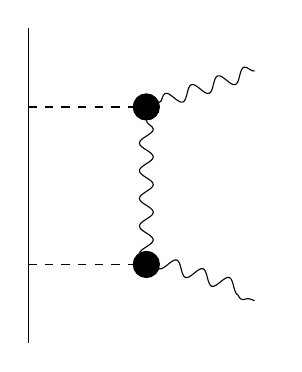
\begin{tikzpicture}

		\begin{scope}		
			\node (A1) at (3,1.5) {};
			\node (A2) at (3,-1.5){};

		\node[circle,draw,fill=black]  (V1) at (1.5,1) {}; 
		\node[circle,draw,fill=black]  (V2) at (1.5,-1) {};  
		\draw[decorate, decoration={snake}]  (V1) --  (A1);
		\draw[decorate, decoration={snake}] (V1) -- (V2) -- (A2);
		\draw[dashed](0,-1) -- (V2);
		\draw[dashed] (0,1) -- (V1);

		\draw (0,2) -- (0,-2);	
	\end{scope}
	\end{tikzpicture}
	\label{fig:orderN}
	\caption{The diagram which encodes the one-loop central term in the OPE.}  
\end{figure}

We proceed with the description of the anomaly associated to the diagram in figure \ref{fig:orderN} which involves two backreaction vertices and a single propagator.
We first consider the terms in the weight of the diagram involving the bulk fields $\mu_1-\mu_2$ (there are also terms involving input fields $\mu-\mu$ and $\alpha-\gamma$).
The weight of this diagram involving these fields is represented by the integral
\beqn
\int_{X,\bfeta_X, Y, \bfeta_Y} \mu_1(X) \, \mu_{BR} (x) \,  \bP (X,Y) \, \mu_{BR}(y) \, \mu_2(Y) ,
\eeqn
where we use coordinates $X = (x_1,x_2,z), Y = (y_1,y_2,w)$ for $\C^3 \times \C^3$ and impose a cutoff $|z-w| \geq \epsilon$.

We first observe the $\eta$-dependence of the integral above.
The backreaction $\mu_{BR}$ is proportional to $F$ and the $\eta$-dependence on the propagator is through $\delta_{\eta_X=\eta_Y}$.
Thus, in total, the $\eta$-dependence on the integrand is
\beqn
\mu_{BR}(\eta_X) \mu_{BR}(\eta_Y) F(\eta_X) F(\eta_Y) \delta_{\eta_X = \eta_Y} .
\eeqn
From this we see that the anomaly associated to this diagram will only involve the unit component of the field $\mu_{BR}(\eta) = \mu_{BR,0} + \cO(\eta)$ and the resulting OPE will be proportional to $N = F^2|_{\eta \br \eta}$.

In appendix \ref{appx:ksbr} we evaluate this integral to obtain
\beqn
 -{N \over 4}  \ep_{ij} \int_{|z-w| \geq \epsilon} \frac{1}{(z-w)^2} \del_{w_i} \mu_1 \del_{w_j} \mu_2|_{w_i=0,\eta=0} .
\eeqn
From this expression, we see that there is a gauge anomaly which can be canceled upon introducing the following term OPE
\beqn
\til J_0^i[1,0](0) \til J_0^j[0,1](z,\what \bfeta') \simeq \cdots \boxed{- \ep^{ij} \frac{1}{4z^2} N} .
\eeqn
The $\cdots$ indicates terms in the OPE which do not depend on the backreaction that we characterized in the previous section (and possibly terms that arise from anomalies associated to other diagrams involving the backreaction, but in this case there are none).

One can use this expression to solve for the OPE involving the on-shell fields.
This central term in the OPE will involve the operators $J[r,s]$ with $r + s = 2$,
which implies that the lowest $\bfeta$-components of such operators comprise an $\lie{sl}(2)$-current algebra of level $N/2$.
For example
\beqn
J_0 [1,1](0) J_0 [1,1] (z) \simeq \frac{1}{z^2} {N \over 2}
\eeqn
where $J_0[1,1]$ is the lowest $\bfeta$-component of the operator $J[1,1]$.

In the previous section, we observed that the tree-level OPE's between the bosonic operators 
\beqn
T_0[0,0], J_0[2,0], J_0[1,1], J_0[0,2]
\eeqn
together with the fermionic operators
\beqn
G_{\alpha,0}[1,0], G_{\alpha,0} [0,1], G_{\gamma,0}[1,0], G_{\gamma,0}[0,1]
\eeqn
comprise the (small) $\cN=4$ superconformal vertex algebra at central charge zero.
We have just seen that the backreaction introduces a level $k = {N \over 2}$ of the $\lie{sl}(2)$ current algebra generated by the fields $J_0[2,0], J_0[1,1], J_0[0,2]$.
This level completely determines the central charge of the superconformal algebra generated by these operators, $c = 12 k = 6 N$.
One can alternatively directly compute the corresponding integrals corresponding to the $TT$ (after putting them on-shell) and $GG$ OPEs and find precisely the remaining central extension terms.

%Since $\mu_{BR}(x)$ only has a $\del_z$-component, and $\mu_{BR}(y)$ only has a $\del_w$ component, we see that the only component of $\bP$ which contributes to this integral is $\del_{x_2} \del_{y_1}$ which reads
%\beqn
%\bP(X,Y)|_{\del_{x_2} \del_{y_1}} = \frac{3}{4 \pi^3 r^8} \eps_{ijk} 
%\eeqn

Notice that by scaling arguments, a central extension to the $JJ$ OPE must take the form $J[k, l]J[r, s] \sim {1 \over z^2}$ (with similar arguments for other possible central extensions). This means the total spin of both generators must add to 4. 
We have presented the calculation when $k + l =2, r + s =2$. 
This is the only combination of spins that impacts the superconformal algebra. 
At the level of unconstrained fields we only considered operators $\til J^i [k,l]$ with $k+l = 1$.
Therefore, the only other possibility we have not yet considered is the OPE between the unconstrained fields $\til J^i [0,0]$ and $\til J^j [1,1]$.
By a completely similar computation, one finds (in the equations below we suppress $\mathcal{O}(1)$ constants, although they can easily be reinstated)
\beqn
\til J^i [0,0](0) \til J^j [1,1](z) \simeq \cdots + \eps^{ij} \frac1{z^2} N .
\eeqn
At the level of the constrained (on-shell) operators, this becomes (up to dropped constants)
\beqn
J[1, 0](0)J[1, 2](z) \sim \cdots + \frac{N}{z^2}
\eeqn
\beqn
J[0, 1](0)J[2, 1](z) \sim \cdots - \frac{N}{z^2}.
\eeqn

\subsection{Non-central effects from backreaction}

We move onto the anomaly arising from the one-loop diagram involving a single backreaction vertex as depicted in figure \ref{fig:oneloopsinglebr}.
In addition to the backreaction, this diagram involves two propagators and a single bulk vertex.

\begin{figure}
	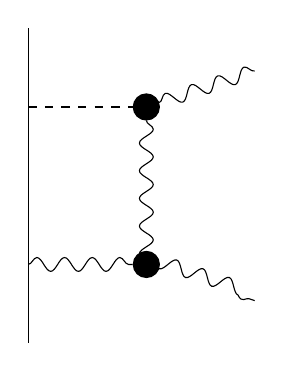
\begin{tikzpicture}

		\begin{scope}		
			\node (A1) at (3,1.5) {};
			\node (A2) at (3,-1.5){};

		\node[circle,draw,fill=black]  (V1) at (1.5,1) {}; 
		\node[circle,draw,fill=black]  (V2) at (1.5,-1) {};  
		\draw[decorate, decoration={snake}]  (V1) --  (A1);
		\draw[decorate, decoration={snake}] (V1) -- (V2) -- (A2);
		\draw[decorate,decoration={snake}](0,-1) -- (V2);
		\draw[dashed] (0,1) -- (V1);

		\draw (0,2) -- (0,-2);	
	\end{scope}
	\end{tikzpicture}
	\label{fig:oneloopsinglebr}
	\caption{This diagram describes the non-central effect of the backreaction.}
\end{figure}

The description of the weight of this diagram is more complicated than the central backreaction terms we have considered so far.
One reason is that this diagram will effect the OPE between an infinite tower of operators in the holographically dual chiral algebra (even in the planar limit).
Secondly, there are more choices of possible labelings of the external edges of this diagram by fields in Kodaira--Spencer theory.

Consider the case where the input fields are $\mu_j$, $j=1,2$ so that the weight of the diagram is represented by the integral
\beqn
\int_{u,\eta_u} \til J^i[a,b](u) \int_{X,\bfeta_X, Y, \bfeta_Y} \left(D_{a,b} \bP (U, X)\right) \mu_j(X) \,  \bP (X,Y) \, \mu_k (Y) \, \mu_{BR} (y)  .
\eeqn
Here $u,\bfeta_U$ are coordinates at the defect vertex and $X,\bfeta_X,Y,\bfeta_Y$ are coordinates at the bulk vertices which we integrate over.
For notational symmetry, we have used the notation $U = (u,0)$ for the viewing the defect coordinate as a bulk coordinate.

The gauge variation of this anomaly is of the form
\beqn
c(i,j,k,l)  \int_{z,\bfeta_u} \left(D_1 \lie{c}_j\right) \del_z^l \left(D_2\mu_k\right) \til J^i [a,b]|_{w=0} \wedge F(\bfeta_u),
\eeqn
where $D_i$ are constant coefficient differential operators (e.g. $D_1 = {1 \over r!}\partial_{w_1}^r$) in the $w_1,w_2$-coordinates whose orders sum to $2l + a + b + 1$, and the $c(i,j,k,l)$ are some coefficients that we compute in Appendix \ref{appx:noncentral}. (We also present the result for a very general one-loop holomorphic integral in Appendix \ref{appx:integral}).
This anomaly will introduce additional linear terms in the OPE between the (off-shell) operators $\til J^j[r,s]$ and $\til J^{k} [r',s']$ of the following heuristic form
\beqn
\til J^j [r,s](0) \til J^k[r',s'] (z) \simeq c'(i,j,k,l) \frac{1}{z^{l+1}} \til J^i[a,b](0) + \cdots
\eeqn
where $r+s+r'+s'=2l+a+b+1$ and the $\cdots$ refer to terms with more derivatives acting on $J^i[a,b]$.



Finally, we remark that the planar chiral algebra should contain the information of the $c=6N$ small $\mathcal{N}=4$ superconformal algebra (which we have reproduced in the OPE of the low-lying generators) as well as OPEs among the superconformal descendants. It would therefore be enlightening to match the Koszul duality approach with more standard bootstrap analyses. This may be slightly tedious, since Koszul duality expresses the chiral algebra in a rather different basis than the one which is natural from the perspective of these symmetries. However, we can readily make certain simple checks. For example, we can verify that our algebra satisfies the $SU(2)_R$ selection rule, valid for the $\mathcal{N}=4$ superconformal algebra with arbitrary central charge, among the OPEs of BPS primaries described on page 7 of \cite{Lin:2015wcg}. We can also use the results of the $\mathcal{N}=4$ long-multiplet bootstrap of \cite{Kos:2018glc}, take the $h \rightarrow (m+n)/2$ limit in which the multiplets become short, and remove the null states, to immediately check that (up to overall numerical factors we did not carefully match) we have obtained the nonvanishing 2-pt functions for the lowest-lying modes; of course, those modes come from nothing but the center of mass multiplet and the $\mathcal{N}=4$ superconformal algebra itself, which we knew from other methods already, but it could be fruitful to apply these checks, and carefully match the results, for the higher modes. 

%\section{Superconformal algebra}
%
%\begin{itemize}
%\item The bosonic operator $T = T^0 [0,0]|_{\bfeta = 0}$ is the stress energy tensor in the superconformal algebra. 
%\item The bosonic operators $J [r,s]|_{\bfeta = 0}$, for $r + s = 2$ comprise the $SU(2)_R$ current.
%Denote $J_0 = J [1,1]|_{\bfeta = 0}$, $J_+ = J^0 [2,0]|_{\bfeta = 0}$, $J_- = J^0[0,2]|_{\bfeta = 0}$. 
%\item The fermionic elements of the superconformal algebra are given by the pair of $SU(2)_R$ doublets 
%\[
%\begin{pmatrix} G_+ \\ \Bar{G}_+ \end{pmatrix} = \begin{pmatrix} \sqrt{2} G^0_\alpha [1,0]|_{\bfeta = 0} \\ \sqrt{2} G^0_\gamma [1,0]|_{\bfeta = 0} \end{pmatrix} , \quad \begin{pmatrix} G_- \\ \Bar{G}_- \end{pmatrix} = \begin{pmatrix} \sqrt{2} G^0_\alpha [0,1]|_{\bfeta = 0} \\ \sqrt{2} G^0_\gamma [0,1]|_{\bfeta = 0} \end{pmatrix}
%\]
%\end{itemize}
%
%
%\subsection{The $TT$ OPE}
%
%In Section \ref{sec:TT1} we computed the tree-level $TT$ OPE at the level of general $w$-descendants.
%Specializing just to $T (z) = T^0[0,0](z)$ we find that the tree-level OPE becomes the usual charge zero Virasoro OPE
%\[
%T(0) T(z) \simeq 2 \frac{1}{z^2} T(0) + \frac{1}{z} \partial_z T(0) .
%\]
%
%At the quantum level, this OPE is deformed. 
%In \S \ref{sec:oneloop} we have shown that there is a one-loop correction to the $\til J \til J$ OPE of the form 
%\[
%\til J^{1}[1,0] (0, \what\bfeta = 0) \til J^{2} [0,1] (z, \what\bfeta'=0) |_{\text{1-loop}} \simeq \frac{N^2}{z^2} .
%\]
%Now, since 
%\[
%T[0,0] (\bfeta) = \til T[0,0] (\bfeta) - \frac12 \left(\del_z \til J^{1}[1,0] (\bfeta) - \del_z \til J^{2}[0,1] (\bfeta) \right) 
%\]
%we see that 
%\[
%T(0) T(z)|_{\text{1-loop}} \simeq \# \del_z^2 \frac{N^2}{z^2} = \# \frac{N^2}{z^4} .
%\]
%
%Here, we note that for type reasons, there is no one-loop quantum correction to the $\til T \til T$ OPE so that the the tree-level plus one-loop $TT$ OPE reads
%\[
%T(0) T(z) \simeq \# \frac{N^2}{z^4} + 2 \frac{1}{z^2} T(0) + \frac{1}{z} \partial_z T(0) .
%\]
%
%
%\subsection{The $JJ$ OPE } 
%
%From \eqref{eqn:TJtree} and we see that the $SU(2)$ currents $J_0, J_\pm$ are weight one primary operators
%\[
%T(0) J_\pm (z) \simeq \frac1z \partial_z J_\pm (0) + \frac{1}{z^2} J_\pm (0) 
%\]
%and similarly for $J_0$. 

\section{Acknowledgments}

NP and VF are supported by funds from the Department of Physics and the College of Arts \& Sciences at the University of Washington, the DOE Early Career Research Program under award DE-SC0022924, and the Simons Foundation as part of the Simons Collaboration in Celestial Holography. NP also thanks Harvard CMSA and the Perimeter Institute's Visiting Fellow program for additional support and hospitality while this work was underway. Research at Perimeter Institute is supported by the Government of Canada through Industry Canada and by the Province of Ontario through the Ministry of Research and Innovation.

\end{document}
